\chapter{Instruction Code Selection \Author{D. Ebner \andAuthor A. Krall \andAuthor B. Scholz} \label{chapter:code_selection}}
\label{chapter:code_selection}
\inputpath[fig]{part4}{code_selection}
\inputprogress

\index{code selection}

% some frequently used macros
%%%%%%%%%%%%%%%%%%%%%%%%%%%%%%%%%%%%%%%%%%%%%%%%%%%%%%%%%%%%%%%%%%%%%
\newcommand{\cf}{c.f.\xspace}
\newcommand{\ea}{et~al.\xspace}

\newcommand{\preds}{\emph{preds}}
\newcommand{\succs}{\emph{succs}}
\newcommand{\costs}{\emph{costs}}
\newcommand{\tbd}[1]{\begin{itemize}\item#1\end{itemize}}
\newcommand\vardomain{\mathbb D}
\newcommand\matrixfont{\mathcal}
\newcommand\kw[1]{\textbf{#1}}

\newcommand\cfgnodes{\mathcal N}
\newcommand\cfgedges{\mathcal E}
\newcommand\cfgstart{\textbf{s}}
\newcommand\cfgend{\textbf{e}}
\newcommand\cfg{\textit{CFG}}
\newcommand\varset{\mathcal{V}}
\newcommand{\vdef}[1]{\cfgdef({#1})}
\newcommand{\defs}[1]{\mathcal{D}_{#1}}
\newcommand{\live}[1]{\mathcal{L}_{#1}}
\newcommand{\uses}[1]{\mathcal{U}_{#1}}
\newcommand{\pred}[2]{\cfgpred^{#1}_{#2}}
\newcommand\state{\textbf{state}}
\newcommand\bool{\mathbb B}
\newcommand\btrue{\textit{true}}
\newcommand\bfalse{\textit{false}}
\newcommand\transform{\mathbb T}
\newcommand\alive{\textbf{alive}}
\newcommand\Path{\textit{Path}}
\newcommand\Ops{\textit{Ops}}
\newcommand\bigo{\mathcal O}

\renewcommand{\vec}[1]{\overrightarrow{#1}}
\newcommand{\dotcup}{\ensuremath{\mathaccent\cdot\cup}}

% locally used colors (pantone)
%%%%%%%%%%%%%%%%%%%%%%%%%%%%%%%%%%%%%%%%%%%%%%%%%%%%%%%%%%%%%%%%%%%%%
\definecolor{LightBlue}{rgb}{ 0.67578125, 0.84375, 0.8984375 }
\definecolor{LightCoral}{rgb}{ 0.9375, 0.5, 0.5 }
\definecolor{LightCyan}{rgb}{ 0.875, 0.99609375, 0.99609375 }
\definecolor{LightGoldenRodYellow}{rgb}{ 0.9765625, 0.9765625, 0.8203125 }
\definecolor{LightGrey}{rgb}{ 0.82421875, 0.82421875, 0.82421875 }
\definecolor{LightGreen}{rgb}{ 0.5625, 0.9296875, 0.5625 }
\definecolor{LightPink}{rgb}{ 0.99609375, 0.7109375, 0.75390625 }
\definecolor{LightSalmon}{rgb}{ 0.99609375, 0.625, 0.4765625 }
\definecolor{LightSeaGreen}{rgb}{ 0.125, 0.6953125, 0.6640625 }
\definecolor{LightSkyBlue}{rgb}{ 0.52734375, 0.8046875, 0.9765625 }
\definecolor{LightSlateBlue}{rgb}{ 0.515625, 0.4375, 0.99609375 }
\definecolor{LightSlateGray}{rgb}{ 0.46484375, 0.53125, 0.59765625 }
\definecolor{LightSteelBlue}{rgb}{ 0.6875, 0.765625, 0.8671875 }
\definecolor{LightYellow}{rgb}{ 0.99609375, 0.99609375, 0.875 }
\definecolor{Orange}{rgb}{ 0.99609375, 0.64453125, 0.0 }
\definecolor{OrangeRed}{rgb}{ 0.99609375, 0.26953125, 0.0 }
\definecolor{Orchid}{rgb}{ 0.8515625, 0.4375, 0.8359375 }

\section{Introduction}

Instruction code selection is a transformation step in a compiler that
translates a machine-independent intermediate code representation into
a low-level intermediate representation or to machine code for a
specific target architecture. Instead of hand-crafting an instruction
selector for each target architecture, generator tools have been
designed and implemented that generate the instruction code selector based
on a specification of the machine description of the
target. This approach is used in large compiler infrastructures such
as GCC or LLVM that target a range of architectures.  A possible
scenario of a code generator in a compiler is depicted in
Figure~\ref{fig:instruction-selection}. The Intermediate
Representation (IR) of an input program is passed on to an optional
lowering phase that breaks down instructions and performs other
machine dependent transformations. Thereafter, the instruction
selection performs the mapping to machine code or lowered IR based on
the machine description of the target architecture.


% \emph{3 pages}; introduction, related work
\begin{figure}[t]
  \begin{center}
    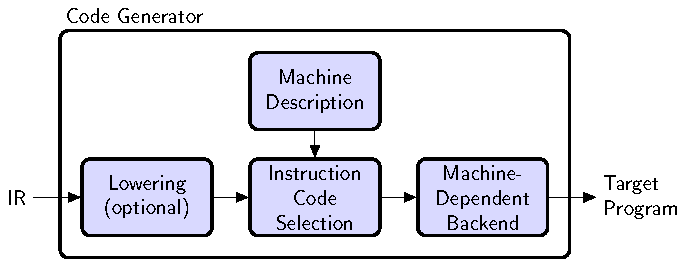
\includegraphics[width=\linewidth]{pgf-fig001}
  \end{center}
  \caption{Scenario: An instruction code selector translates a compiler's IR to a
    low-level machine-dependent representation.}
  \label{fig:instruction-selection}
\end{figure}

One of the widely used techniques in code generation is tree pattern
matching\index{pattern matching}. The unit of translation for tree pattern matching is 
expressed as a tree structure
that is called a data-flow tree\index{data-flow tree, DFT} (DFT). 
The basic idea is
to describe the target instruction set using an \emph{ambiguous}
cost-annotated graph grammar\index{grammar}. The instruction code selector seeks for a
cost-minimal \emph{cover} of the DFT. Each of the selected rules have
an associated semantic action that is used to emit the corresponding
machine instructions, either by constructing a new intermediate
representation or by rewriting the DFT bottom-up.
\begin{figure}[ht]
  \begin{center}
    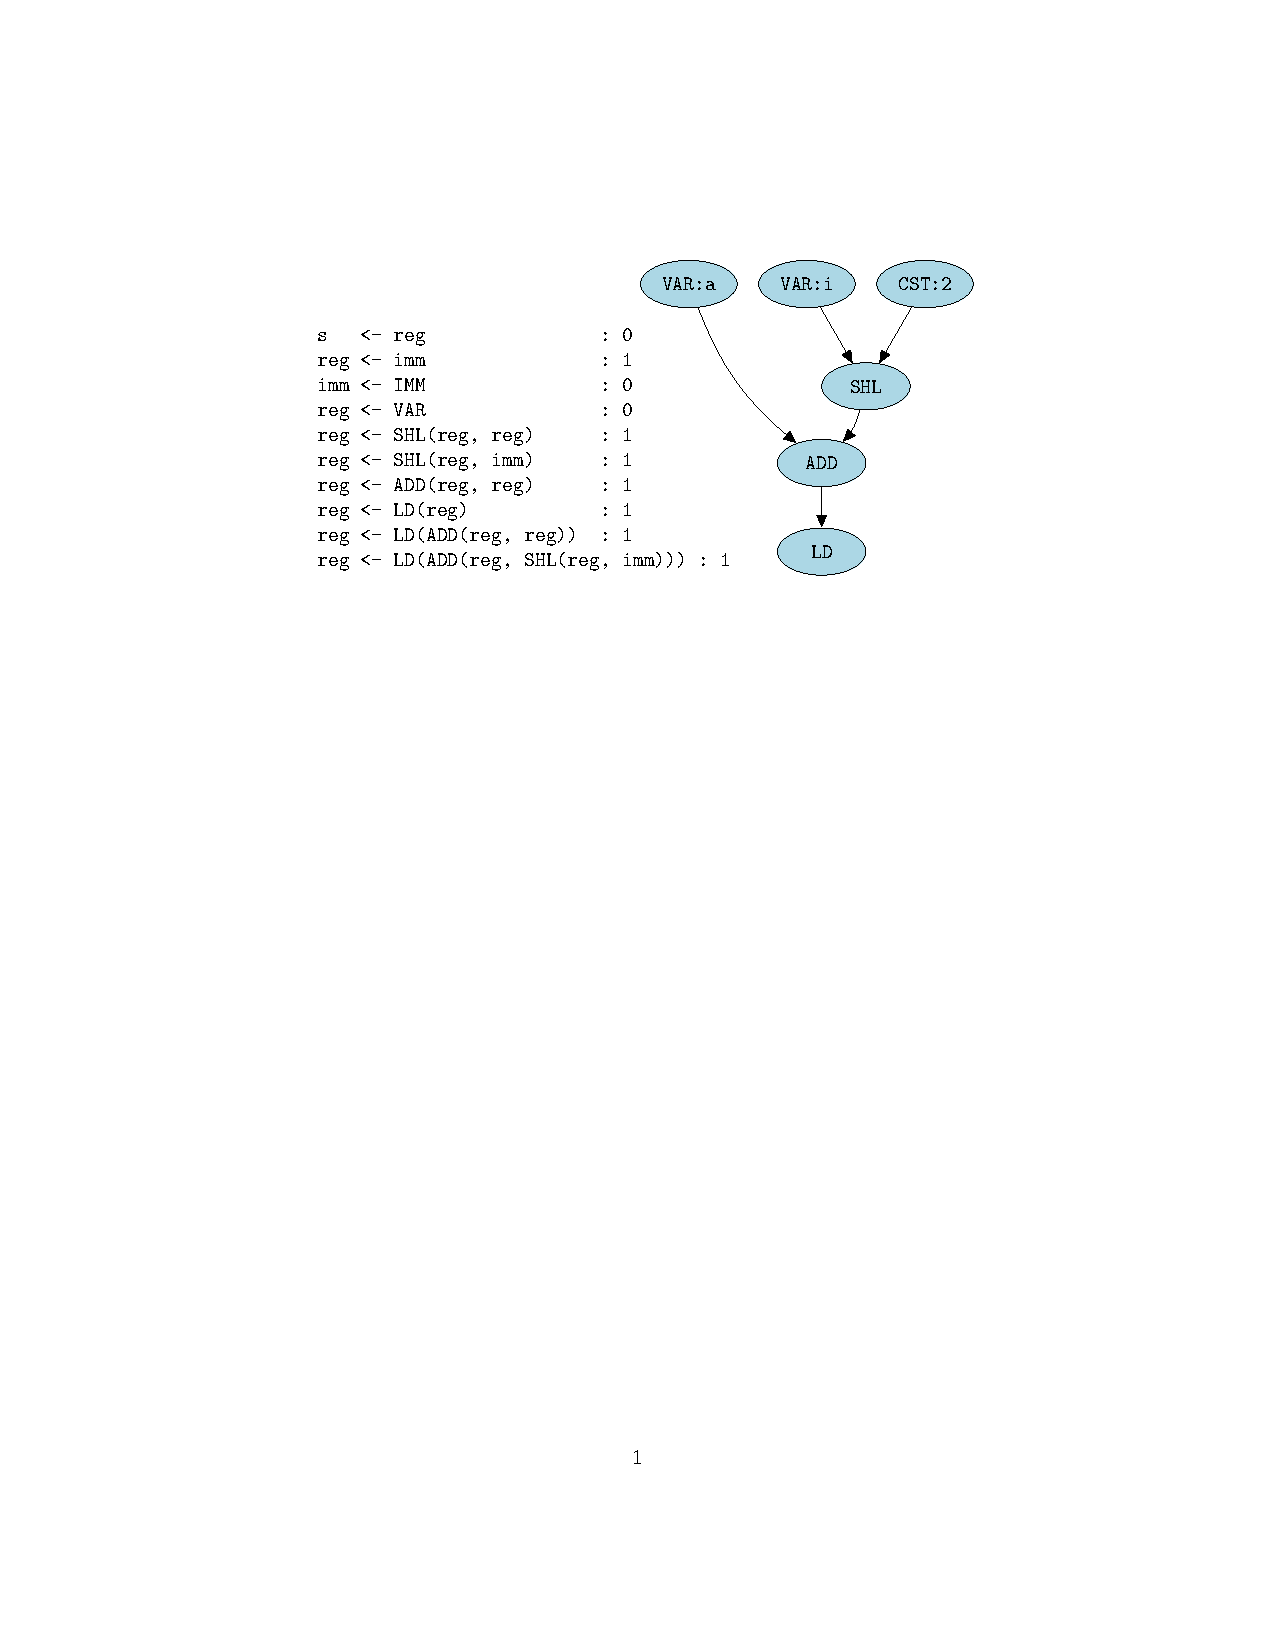
\includegraphics[scale=0.9]{pgf-fig002}
  \end{center}
  \caption{Example of a data-flow tree and a rule fragment with
    associated costs.}\label{fig:tpm}
%TODO: number the rules from 1 to 11
\end{figure}

An example of a DFT along with a set of rules representing valid ARM
instructions is shown in Figure~\ref{fig:tpm}. Each rule consists of
non-terminals\index{symbol, non-terminal} (shown in lower-case), and terminal symbols\index{symbol, terminal} (shown in
upper-case). Non-terminals are used to chain individual rules together.
Non-terminal \texttt{s} denotes a distinguished start symbol for the
root node of the DFT. Terminal symbols match the corresponding labels
of nodes in the data-flow trees. The terminals of the grammar are
\texttt{VAR}, \texttt{CST}, \texttt{SHL}, \texttt{ADD}, and
\texttt{LD}.  Rules that translate from one non-terminal to another are
called \emph{chain rules}\index{rule, chain}, e.g., \texttt{reg $\gets$ imm} that translates
an immediate value to a register. Note that there are multiple
possibilities to obtain a cover of the data-flow tree for the example
shown in Figure~\ref{fig:tpm}.  Each rule has associated costs. The
cost of a tree cover is the sum of the costs of the selected
rules. For example, the DFT could be covered by rules $R_3$, $R_4$, and~$R_{10}$ which would give a total cost for the cover of one cost
unit. Alternatively, the DFT could be covered by rule $R_2$, $R_3$, $R_5$, $R_7$, and~$R_8$ which yields four cost units for the cover for issuing four assembly
instructions. A dynamic programming algorithm selects a cost optimal
cover for the DFT.


Tree pattern matching on a DFT is limited to the scope of tree
structures.  To overcome this limitation, we can extend the scope of
the matching algorithm to the computational flow of a whole procedure.
The use of the SSA form as an intermediate
representation improves the code generation by making def-use\index{def-use chains}
relationships explicit. Hence, SSA exposes the data flow of a
translation unit and utilizes the code generation process.  Instead of
using a textual SSA representations, we employ a graph representation
of SSA called the \emph{SSA graph}~\footnote{We consider its
  data-based representation here.\index{SSA graph, data-based} See Chapter~\ref{chapter:vsdg}} that
is an extension of DFTs and represents the data flow for scalar
variables of a procedure in SSA form.  SSA graphs are a suitable
representation for code generation: First, SSA graphs capture acyclic
and cyclic information flow beyond basic block boundaries. Second, SSA
graphs often arise naturally in modern compilers as the intermediate
code representation usually already is in SSA form. Third, output or
anti-dependencies in SSA graph do not exist.

As even acyclic SSA graphs are in the general case not restricted to a tree, no dynamic programming approach
can be employed for instruction code selection.  To get a handle on instruction code
selection for SSA graphs, we will discuss in the following an approach
based on a reduction to a quadratic mathematical programming problem
(PBQP).  Consider the code fragment of a dot-product routine
and the corresponding SSA graph shown in Figure~\ref{fig:ssa_graph}.
The code implements a simple vector dot-product using fixed-point\index{fixed-point arithmetic}
arithmetic.  Nodes in the SSA graph represent a single
operation while edges describe the flow of data that is produced at the
source node and consumed at the target node. Incoming edges
have an order which reflects the argument order of the operation. In
the figure the color of the nodes indicates to which basic block the
operations belong to.

\begin{figure}[bh]
  \begin{center}
%TODO: if we remove the colors, change the text accordingly below
   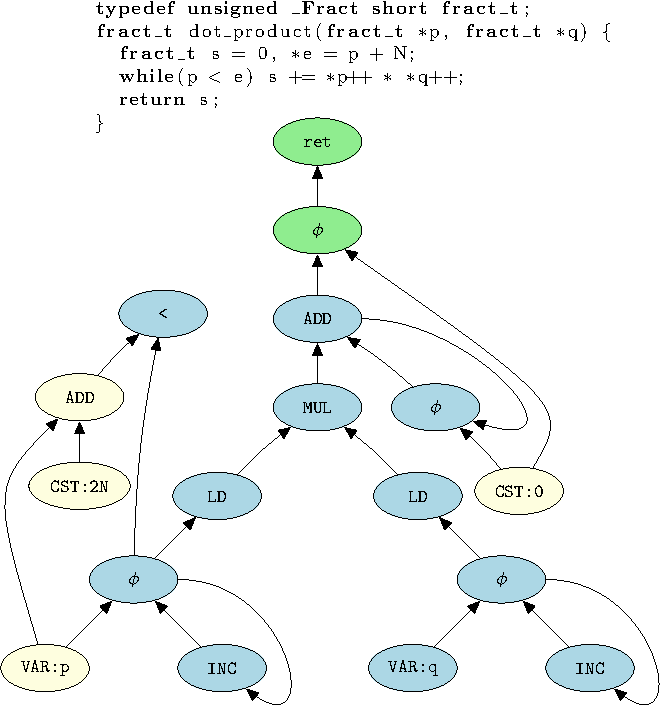
\includegraphics[width=1.03\textwidth]{pgf-fig003}
  \end{center}
  \caption{Instruction code selection SSA Graph for a vector dot-product in
    fixed-point arithmetic.  \texttt{fp\_} stands for unsigned short fixed point type. }\label{fig:ssa_graph}
\end{figure}

The example in Figure~\ref{fig:ssa_graph} has fixed-point computations
that need to be modeled in the grammar. For fixed-point values most
arithmetic and bit-wise operations are identical to their integer
equivalents. However, some operations have different semantics, \eg
multiplying two fixed-point values in format $m.i$ results in a value
with $2i$ fractional digits. The result of the multiplication has to
be adjusted by a shift operation to the right (\texttt{LSR}). To accommodate for
fixed-point values, we add the following rules to the grammar
introduced in Figure~\ref{fig:tpm}:
\begin{center}
\begin{tabular}{l|l|l}
  rule & cost & instruction\\ \hline
   \tt reg $\gets$ VAR & is\_fixed\_point ? \(\infty\) otherwise 0\\
   \tt fp \ $\gets$ VAR & is\_fixed\_point ? 0 \ otherwise  \(\infty\)  \\
  \tt  fp2 $\gets$ MUL(fp, fp)   & 1 & \tt   MUL Rd, Rm, Rs \\
  \tt  fp \ $\gets$ fp2           & 1 &\tt   LSR Rd, Rm, i  \\
  \tt  fp \ $\gets$ ADD(fp, fp)   & 1 & \tt   ADD Rd, Rm, Rs \\
  \tt  fp2 $\gets$ ADD(fp2, fp2) & 1 & \tt   ADD Rd, Rm, Rs \\
  \tt  fp \ $\gets$ PHI(fp, ...) & 0 \\
  \tt  fp2 $\gets$ PHI(fp2, ...) & 0 \\
\end{tabular}
\end{center}

In the example the accumulation for double-precision fixed
point values (\texttt{fp2}) can be performed at the same cost as for the single-precision format (\texttt{fp}). Thus, it would be
beneficial to move the necessary shift from the inner loop to the
return block, performing the intermediate calculations in the extended
format. However, as a tree-pattern matcher generates code at 
statement-level, the information of having values as double-precision
cannot be hoisted across basic block boundaries.
An instruction code selector that is operating on the SSA graph, is able to propagate 
non-terminal \texttt{fp2} across the $\phi$ node prior to the return 
and emits the code for the shift to the right in the return block.

In the following, we will explain how to perform instruction code selection
on SSA graphs with the means of a specialized quadratic assignment
problem (PBQP). First, we discuss the instruction code selection problem by
employing a discrete optimization problem called partitioned boolean
quadratic problem.  An extension of \emph{patterns} to arbitrary
acyclic graph structures, which we refer to as DAG grammars, is
discussed in Sub-Section~\ref{sec:dag_patterns}.

\section{Instruction Code Selection for Tree Patterns on SSA-Graphs}
% \emph{5 pages}; modeling, continued example
The matching problem for SSA graphs reduces to a discrete optimization
problem called Partitioned Boolean Quadratic Problem (PBQP).  First,
we will introduce the PBQP problem and then we will describe the
mapping of the instruction code selection problem to PBQP.

\subsection{Partitioned Boolean Quadratic Problem}
\label{sec:pbqp}\index{Partitioned Boolean Quadratic Programming, PBQP}
% \emph{2 pages}; introduction into PBQP, algorithms, and applications
Partitioned Boolean Quadratic Programming (PBQP) is a generalized
quadratic assignment problem that has proven to be effective for a
wide range of applications in embedded code generation, \eg
register assignment, address mode selection, or
bank selection for architectures with partitioned memory. Instead of
problem-specific algorithms, these problems can be modeled in terms of
generic {PBQP}s that are solved using a common solver library. PBQP is
flexible enough to model irregularities of embedded architectures that
are hard to cope with using traditional heuristic approaches.

Consider a set of discrete variables $X=\{x_1,\ldots,x_n\}$ and their
finite domains $\{\vardomain_1,\ldots,\vardomain_n\}$. A solution of
PBQP is a mapping $h$ of each variable to an element in its domain,
i.e., an element of $\vardomain_i$ needs to be chosen for variable
$x_i$. The chosen element imposes \emph{local costs} and \emph{related costs} with
neighboring variables.  Hence, the
quality of a solution is based on the contribution of two sets of
terms.
\begin{enumerate}
\item For assigning variable $x_i$ to the element $d_i$ in
  $\vardomain_i$. The quality of the assignment is measured by a
  \emph{local cost function} $c(x_i, d_i)$.
\item For assigning two related variables $x_i$ and $x_j$ to the
  elements $d_i \in \vardomain_i$ and $d_j \in \vardomain_j$.  We
  measure the quality of the assignment with a \emph{related cost
    function\/} $C(x_i,x_j, d_i,d_j)$.
\end{enumerate}
The total cost of a solution $h$ is given as,
\begin{equation}
  f\! =\! \sum_{1 \leq i \leq n} \hspace{-1mm} c(x_i,h(x_i)) + \hspace{-3mm} \sum_{1 \leq i < j  \leq n} \hspace{-3.5mm}
  C\left (x_i,x_j, h(x_i), h(x_j) \right). \label{eqn-pbqp}
\end{equation}
The PBQP problem seeks for an assignment of variables $x_i$ with
minimum total costs.

In the following we represent both the local cost function and the
related cost function in matrix form, i.e., the related cost function
$C(x_i,x_j,d_i,d_j)$ is decomposed for each pair $(x_i,x_j)$. The
costs for the pair are represented as $|\vardomain_i|\textrm{-by-}|\vardomain_j|$ matrix/table ${\matrixfont
  C}_{ij}$. A matrix element corresponds to an assignment $(d_i,
d_j)$. Similarly, the local cost function $c(x_i,d_i)$ is represented
by a cost vector $\vec{c_i}$ enumerating the costs of the elements.  A
PBQP problem has an underlying graph structure graph $G=(V,E,C,c)$,
which we refer to as a PBQP graph. For each decision variable $x_i$ we
have a corresponding node $v_i \in V$ in the graph, and for each cost
matrix ${\matrixfont C}_{i,j}$ that is not the zero matrix, we
introduce an edge $e=(v_i,v_j)$. The cost functions $c$ and $C$ map
nodes and edges to the original cost vectors and matrices
respectively.  We will present an example later in this chapter in the
context of instruction code selection.

In general, finding a solution to this minimization problem is NP
hard.  However, for many practical cases, the PBQP instances are
sparse, \ie many of the cost matrices ${\matrixfont C}_{i,j}$ are zero
matrices and do not contribute to the overall solution. Thus, optimal
or near-optimal solutions can often be found within reasonable time
limits.  Currently, there are two algorithmic approaches for PBQP that
have been proven to be efficient in practice for instruction code selection
problems, \ie a polynomial-time heuristic algorithm and a
branch-\&-bound based algorithm with exponential worst case
complexity.  For a certain subclass of PBQP, the algorithm produces
provably optimal solutions in time ${\cal O}(n m^3)$, where $n$ is the
number of discrete variables and $m$ is the maximal number of elements
in their domains, \ie $m=\max
\left(|\vardomain_1|,\ldots,|\vardomain_n\right|)$. For general
{PBQP}s, however, the solution may not be optimal. To obtain still an
optimal solution outside the subclass, branch-\&-bound techniques can
be applied.

\subsection{Instruction Code Selection with PBQP}
In the following, we describe the modeling of instruction code selection for SSA
graphs as a PBQP problem.  In the basic modeling, SSA and PBQP graphs
coincide.  The variables $x_i$ of the PBQP are decision variables
reflecting the choices of applicable rules (represented by
$\vardomain_i$) for the corresponding node of $x_i$. The local costs
reflect the costs of the rules and the related costs reflect the costs
of chain rules making rules compatible with each other.  This means
that the number of decision vectors and the number of cost matrices in
the PBQP are determined by the number of nodes and edges in the SSA
graph respectively.  The sizes of $\vardomain_i$ depend on the number
of rules in the grammar. A solution for the PBQP instance induces a
complete cost minimal cover of the SSA graph.

As in traditional tree pattern matching, an ambiguous graph grammar
consisting of tree patterns with associated costs and semantic actions
is used. Input grammars have to be \emph{normalized}. This means that
each rule is either a so-called \emph{base rule} or a \emph{chain  rule}. A base rule\index{rule, base} is a production of the form $\texttt{nt}_0
\leftarrow \textit{OP} ( \texttt{nt}_1, \dots, \texttt{nt}_{k_p} )$
where $\texttt{nt}_i$ are non-terminals and $\textit{OP}$ is a
terminal symbol, \ie an operation represented by a node in the SSA
graph. A chain-rule is a production of the form $\texttt{nt}_0
\leftarrow \texttt{nt}_1$, where $\texttt{nt}_0$ and $\texttt{nt}_1$
are non-terminals.  A production rule\index{rule, production} $\texttt{nt} \leftarrow
\textit{OP}_1 ( \alpha, \textit{OP}_2 (\beta), \gamma))$ can be
normalized by rewriting the rule into two production rules
$\texttt{nt} \leftarrow \textit{OP}_1 ( \alpha, \texttt{nt}' ,
\gamma)$ and $\texttt{nt}' \leftarrow \textit{OP}_2 ( \beta)$ where
$\texttt{nt}'$ is a new non-terminal symbol and $\alpha,\beta$ and
$\gamma$ denote arbitrary pattern fragments.  This transformation can
be iteratively applied until all production rules are either chain
rules or base rules.  To illustrate this transformation, consider the
grammar in Figure~\ref{fig:pbpq-example}, which is a normalized
version of the tree grammar introduced in
Figure~\ref{fig:tpm}. Temporary non-terminal symbols $\texttt{t1}$,
$\texttt{t2}$, and $\texttt{t3}$ are used to decompose larger tree
patterns into simple base rules. Each base rule spans across a single
node in the SSA graph.


\begin{figure}
  \begin{center}
    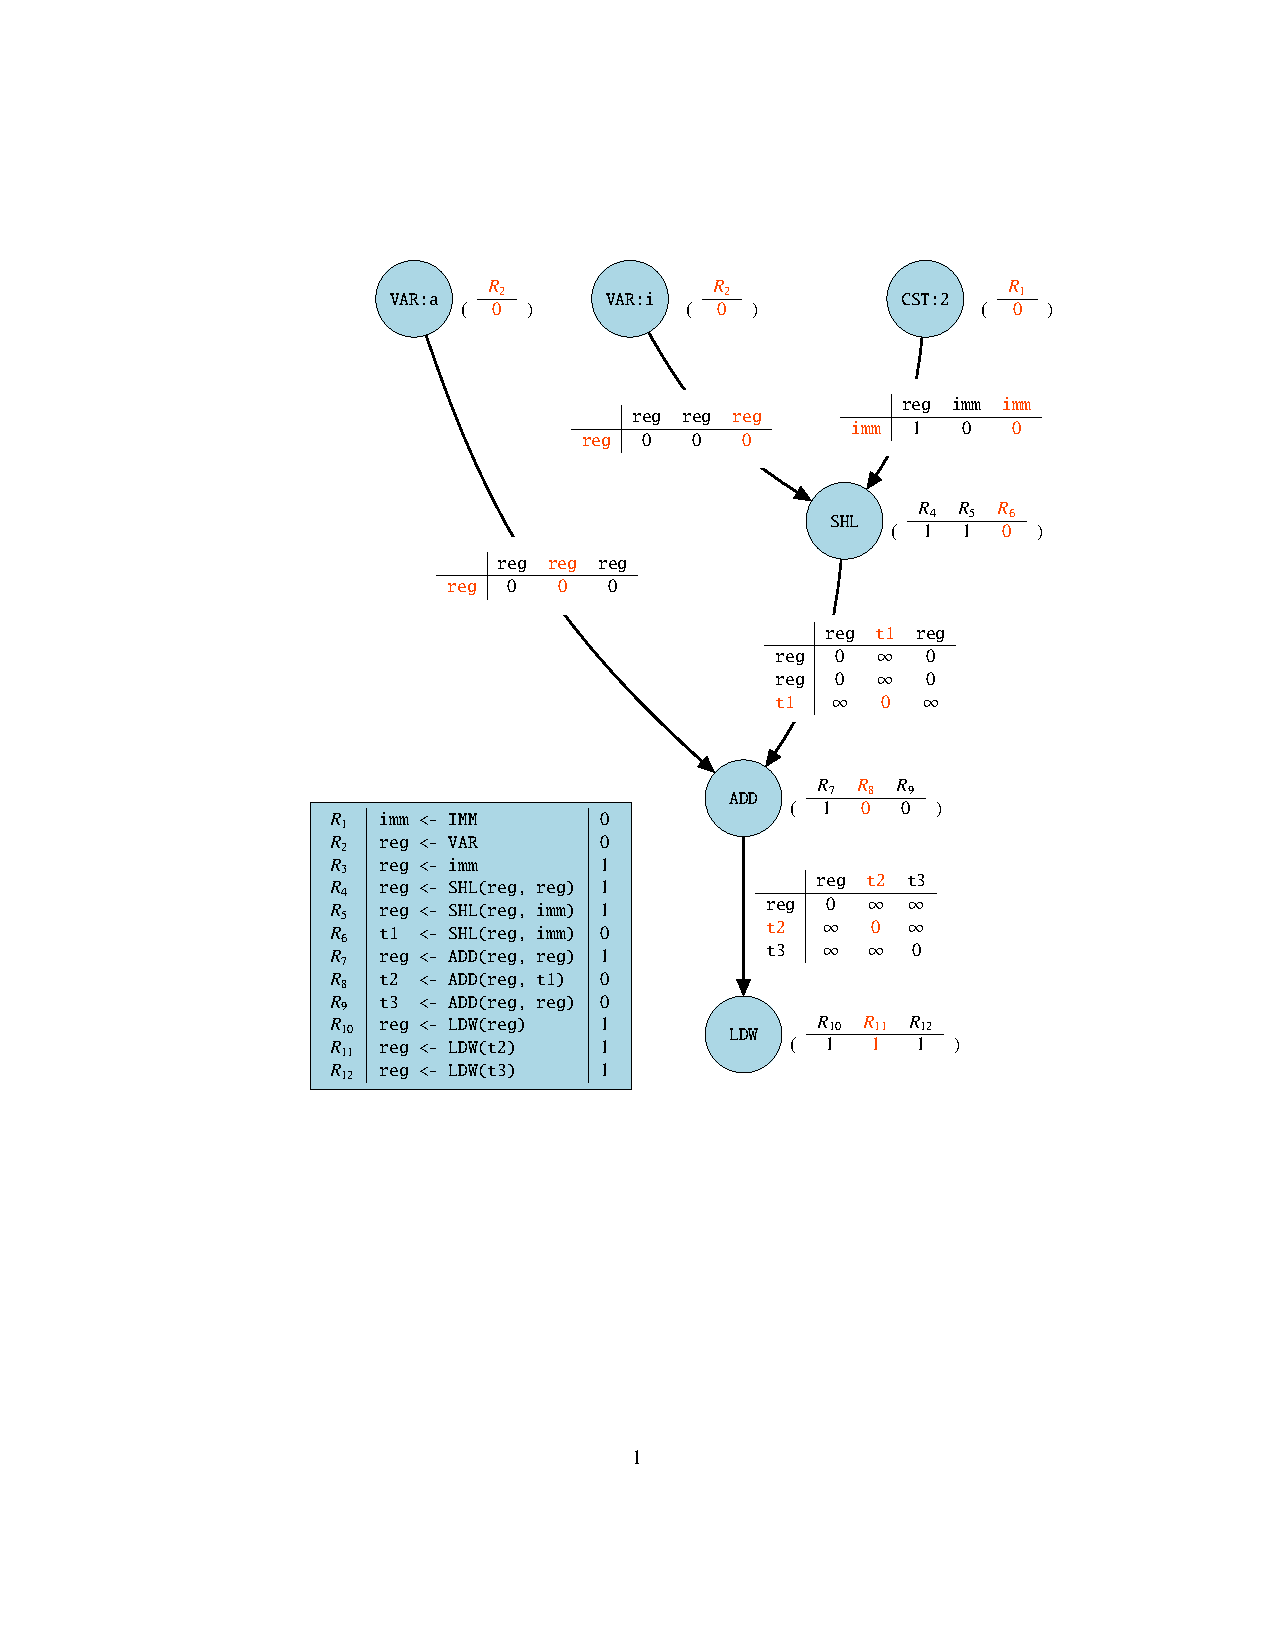
\includegraphics[width=\linewidth]{pgf-fig006}
  \end{center}
  \caption{PBQP instance derived from the example shown in
    Figure~\ref{fig:tpm}. The grammar has been normalized by
    introducing additional non-terminals.}\label{fig:pbpq-example}
\end{figure}


The instruction code selection problem for SSA graphs is modeled in PBQP as
follows. For each node $u$ in the SSA graph, a PBQP variable $x_u$ is
introduced. The domain of variable $x_u$ is determined by the subset
of base rules whose terminal symbol matches the operation of the SSA
node, \eg there are three rules ($R_4$, $R_5$, $R_6$) that can be
used to cover the shift operation $\texttt{SHL}$ in our example. The
last rule is the result of automatic normalization of a more complex
tree pattern.
The cost vector $\vec{c_u}= w_u \cdot \langle c(R_1), \dots,
c(R_{k_u}) \rangle$ of variable $x_u$ encodes the local costs for a
particular assignment where $c(R_i)$ denotes the associated cost of
base rule $R_i$. Weight $w_u$ is used as a parameter to optimize for
various objectives including speed (e.g., $w_u$ is the expected
execution frequency of the operation at node $u$) and space (e.g., the
$w_u$ is set to one). In our example, both $R_4$ and $R_5$ have
associated costs of one. Rule $R_6$ contributes no local costs as we
account for the full costs of a complex tree pattern at the root
node. All nodes have the same weight of one, thus the cost vector for
the \texttt{SHL} node is $\langle1, 1, 0 \rangle$.

An edge in the SSA graph represents data transfer between the result
of an operation $u$, which is the source of the edge, and the operand
$v$ which is the tail of the edge.  To ensure consistency among base
rules and to account for the costs of chain rules, we impose costs
dependent on the selection of variable $x_u$ and variable $x_v$ in the
form of a cost matrix $\matrixfont C_{uv}$. An element in the matrix
corresponds to the costs of selecting a specific base rule $r_u \in
R_u$ of the result and a specific base rule $r_v \in R_v$ of the
operand node. Assume that $r_u $ is $\texttt{nt} \leftarrow
\textit{OP} (\dots)$ and $r_v$ is $\dots \leftarrow \textit{OP}
(\alpha, \texttt{nt}', \beta)$ where $\texttt{nt}'$ is the
non-terminal of operand $v$ whose value is obtained from the result of
node $u$. There are three possible cases:
\begin{enumerate}
\item If the non-terminal \texttt{nt} and \texttt{nt}' are identical,
  the corresponding element in matrix $\matrixfont C_{uv}$ is zero,
  since the result of $u$ is compatible with the operand of node $v$.
\item If the non-terminals \texttt{nt} and $\texttt{nt}'$ differ and
  there exists a rule $r: \texttt{nt}' \leftarrow \texttt{nt}$ in the
  transitive closure of all chain rules, the corresponding element in
  $\matrixfont C_{uv}$ has the costs of the chain rule, \ie $w_v \cdot
  c(r)$.
\item Otherwise, the corresponding element in $\matrixfont C_{uv}$ has
  infinite costs prohibiting the selection of incompatible base rules.
\end{enumerate}

As an example, consider the edge from \texttt{CST:2} to node
\texttt{SHL} in Figure~\ref{fig:pbpq-example}. There is a single base
rule $R_1$ with local costs 0 and result non-terminal \texttt{imm} for
the constant. Base rules $R_4$, $R_5$, and $R_6$ are applicable for
the shift, of which the first one expects non-terminal \texttt{reg} as
its second argument, rules $R_5$ and $R_6$ both expect
\texttt{imm}. Consequently, the corresponding cost matrix accounts for
the costs of converting from \texttt{reg} to \texttt{imm} at index
$(1,1)$ and is zero otherwise.

Highlighted elements in Figure~\ref{fig:pbpq-example} show a
cost-minimal solution of the PBQP with costs one. A solution of the
PBQP directly induces a selection of base and chain rules for the SSA
graph. The execution of the semantic action rules inside a basic block
follow the order of basic blocks. Special care is necessary for chain rules 
that link data flow across basic blocks. Such chain rules may be placed
inefficiently and a placement algorithm~\cite{1269857} is required for
some grammars. 

\section{Extensions and Generalizations}

\subsection{Instruction Code Selection for DAG Patterns}
% TODO (continue here)
\label{sec:dag_patterns}
% generalization for DAG patterns; motivation; modeling; example
In the previous section we have introduced an approach based on code
patterns that resemble simple tree fragments. This restriction often
complicates code generators for modern CPUs with specialized
instructions and SIMD extensions, \eg there is no support for
machine instructions with multiple results.

Consider the introductory example shown
in Figure~\ref{fig:ssa_graph}. Many architectures have some form of
auto-increment addressing modes. On such a machine, the load and the
increment of both \texttt{p} and \texttt{q} can be done in a single
instruction benefiting both code size and performance. However,
post-increment loads cannot be modeled using a single tree-shaped
pattern. Instead, it produces multiple results and spans across two
non-adjacent nodes in the SSA graph, with the only restriction that
their arguments have to be the same.

Similar examples can be found in most architectures, \eg the
\texttt{DIVU} instruction in the Motorola 68K architecture performs
the division and the modulo operation for the same pair of
inputs. Other examples are the \texttt{RMS} (read-modify-store)
instructions on the IA32/AMD64 architecture, autoincrement- and
decrement addressing modes of several embedded systems architectures,
the \texttt{IRC} instruction of the HPPA architecture, or
\texttt{fsincos} instructions of various math libraries. Compiler
writers are forced to pre- or post-process these patterns
heuristically often missing much of the optimization potential. 
These architecture-specific tweaks also complicate
re-targeting, especially in situations where patterns are
automatically derived from generic architecture descriptions.


\begin{figure}[t]
  \centering
  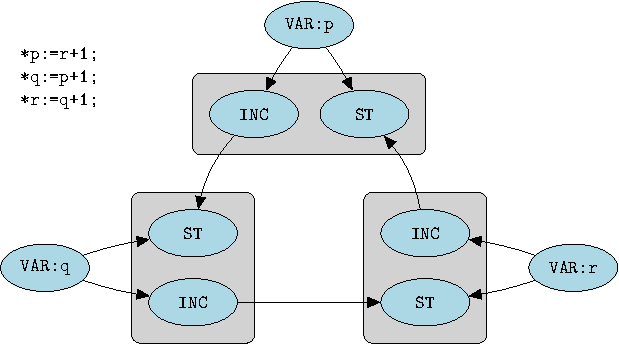
\includegraphics[scale=0.9]{pgf-fig008}
  \caption{DAG patterns may introduce cyclic data dependencies.}\label{fig:topology}
\end{figure}

We will now outline, through the example in
Figure~\ref{fig:topology}, a possible problem formulation for these
generalized patterns in the PBQP framework discussed so far. 
The code fragment contains three feasible instances of a post-increment
store pattern. Assuming that $p$, $q$, and $r$ point to mutually
distinct memory locations, there are no further dependencies apart
from the edges shown in the SSA graph. If we select \emph{all } three
instances of the post-increment store pattern concurrently, the graph induced by SSA edges becomes acyclic, and the code cannot be emitted. To overcome this difficulty, the idea is to express in the modeling of the problem, a numbering of chosen nodes, that reflects the existence of a topological order. 


\paragraph{Modeling}
The first step is to explicitly enumerates \emph{instances\/} of complex
patterns, \ie
concrete tuples of nodes that match the terminal symbols specified in
a particular production. There are three instances of the
post-increment store pattern (surrounded by boxes) in the example shown
in Figure~\ref{fig:topology}.
As for tree patterns, DAG patterns are decomposed into simple base
rules for the purpose of modeling, \eg the post-increment store
pattern
\begin{alltt}
  \(P\sb{1}\): tmt \(\gets\) ST(\(x\):reg, reg), reg \(\gets\) INC(\(x\)) : 3
\end{alltt}
is decomposed into the individual pattern fragments
\begin{alltt}
  \(P\sb{1,1}\): stmt \(\gets\) ST(reg, reg)
  \(P\sb{1,2}\): reg  \(\gets\) INC(reg)
\end{alltt}

For our modeling, new variables are created for each enumerated
instance of a complex production. They encode whether a particular
instance is chosen or not, \ie the domain basically consists of the
elements \texttt{on} and \texttt{off}. The local costs are set to the
combined costs for the particular pattern for the \texttt{on} state
and to 0 for the \texttt{off} state. Furthermore, the domain of
existing nodes is augmented with the base rule fragments obtained from
the decomposition of complex patterns.  We can safely squash all
identical base rules obtained from this process into a single
state. Thus, each of these new states can be seen as a proxy for the
whole set of instances of (possibly different) complex productions
including the node. The local costs for these proxy states are set to 0.

\begin{figure}
  \centering
    ~\hspace{-2cm}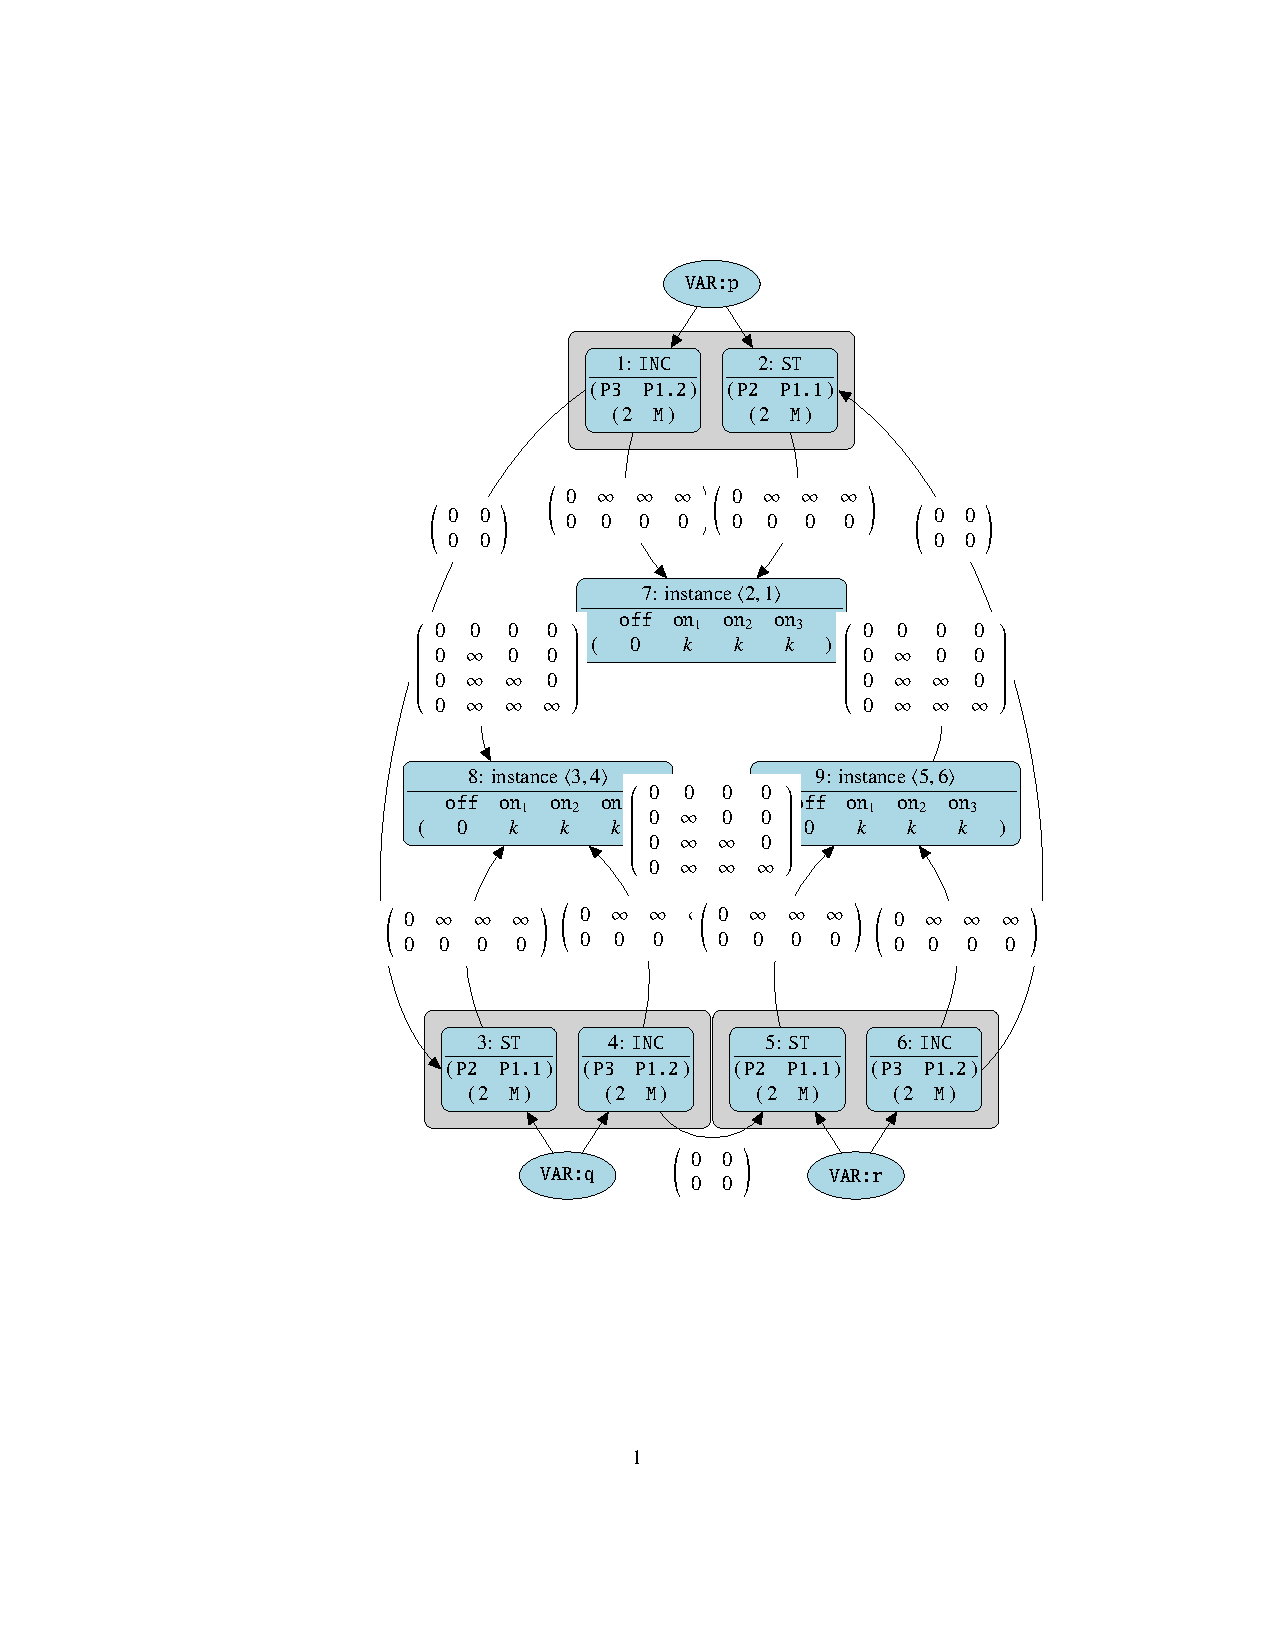
\includegraphics[width=1.33\textwidth]{pgf-fig009}
  \caption{PBQP Graph for the Example shown in
    Figure~\ref{fig:topology}. $M$ is a large integer value. We use $k$ as a shorthand for the term
    $3-2M$.}\label{fig:pbqpinst}
\end{figure}

Continuing our example, the PBQP for the SSA graph introduced in
Figure~\ref{fig:topology} is shown in Figure~\ref{fig:pbqpinst}. In
addition to the post-increment store pattern with costs three, we assume
regular tree patterns for the store and the increment nodes with costs
two denoted by $P_2$ and $P_3$ respectively. Rules for the
\texttt{VAR} nodes are omitted for simplicity.

Nodes 1 to 6 correspond to the nodes in the SSA graph. Their
domain is defined by the simple base rule with costs two and the proxy
state obtained from the decomposition of the post-increment store
pattern. Nodes~7, 8, and~9 correspond to the three instances
identified for the post-increment store pattern. As noted before, we
have to guarantee the existence of a topological order among the
chosen nodes. To this end, we refine the state \texttt{on} such that it
reflects a particular index in a concrete topological order. Matrices
among these nodes account for data dependencies, \eg consider the
matrix established among nodes~7 and~8. Assuming instance~7 is
\texttt{on} at index~2 (i.e., mapped to $\texttt{on}_2$), the only remaining choices for instance~8 are
not to use the pattern (i.e., mapped to \texttt{off}) or to enable it at index~3 (i.e., mapped to $\texttt{on}_3$), as node~7 has
to precede node~8.

Additional cost matrices are required to ensure that the corresponding
proxy state is selected on all the variables forming a particular
pattern instance (which can be modeled with combined costs of 0 or
$\infty$ respectively). However, this formulation allows for the
trivial solution where all of the related variables encoding the
selection of a complex pattern are set to \texttt{off} (accounting for
0 costs) even though the artificial proxy state has been selected. We
can overcome this problem by adding a large integer value $M$ to the
costs for all proxy states. In exchange, we subtract these costs from
the cost vector of instances. Thus, the penalties for the proxy states
are effectively eliminated unless an invalid solution is selected.

Cost matrices among nodes 1 to 6 do not differ from the basic
approach discussed before and reflect the costs of converting the
non-terminal symbols involved.  It should be noted that for general
grammars and irreducible graphs, that the heuristic solver of PBQP
cannot guarantee to deliver a solution that satisfies all constraints
modeled in terms of $\infty$ costs. This would be a NP-complete
problem. One way to work around this limitation is to include a small
set of rules that cover each node individually and that can be used as
a fallback rule in situations where no feasible solution has been
obtained, which is similar to macro substitution techniques and
ensures a correct but possibly non-optimal matching. These limitations
do not apply to exact PBQP solvers such as the branch-\&-bound
algorithm. It is also straight-forward to extend the heuristic
algorithm with a backtracking scheme on RN reductions, which would of
course also be exponential in the worst case.

%%%FAB: extremely difficult to understand as it is and not very useful
%% \paragraph{Algorithm}
%% \LinesNumbered
%% \begin{algorithm}
  %% identify instances of complex patterns within basic blocks\;
  %% transform the problem to an instance of PBQP\;
  %% obtain a solution for the PBQP instance using a generic solver\;
  %% \ForAll{basic blocks $b$} {
    %% compute a topological order for the sub-graph induced by $b$\;
    %% apply semantic rules associated with the chosen productions\;
  %% }
  %% \caption{\label{alg:pbqpisel}Generalized PBQP instruction code selection}
%% \end{algorithm}

%% Algorithm~\ref{alg:pbqpisel} outlines the generalized algorithm in
%% pseudo-code. Only lines \texttt{(1)}, \texttt{(2)}, and \texttt{(5)}
%% differ from the approach discussed so far. First, we identify concrete
%% tuples of nodes in the SSA graph that can be used to form complex
%% patterns. Next, we transform the problem to an instance of PBQP that
%% is processed using a generic solver library. The problem formulation
%% ensures the existence of a topological order among the chosen
%% productions and allows for a straight-forward back-transformation that
%% maps a solution vector of PBQP to a complete graph cover. The partial
%% order among the particular nodes is defined by the edges in the SSA
%% graph and additional data dependencies among load and store
%% instructions.  We can thus use a reversed post-order traversal to
%% apply the semantic actions associated with the chosen productions in a
%% proper order on the sub-graphs induced by individual basic blocks.

\section{Summary and Further Reading}
Aggressive optimizations for the instruction code selection problem are enabled by the use of SSA graph.
The whole flow of a function is taken into account
rather a local scope. The move from basic tree-pattern
matching~\cite{aj:76} to SSA-based DAG matching is a relative small
step as long as a PBQP library and some basic infrastructure (graph
grammar translator, etc.)  is provided. The complexity of the approach
is hidden in the discrete optimization problem called PBQP. Free PBQP
libraries are available from the web-pages of the authors and a
library is implemented as part of the LLVM~\cite{wwwLLVM} framework.

Many aspects of the PBQP formulation presented in this chapter could
not be covered in detail. The interested reader is referred to the
relevant literature~\cite{EcksteinKS03,Ebner08} for an in-depth
discussion.

As we move from acyclic linear code regions to whole-functions, it
becomes less clear in which basic block, the selected machine
instructions should be emitted. For chain rules, the obvious choices
are often non-optimal. In~\cite{1269857}, a polynomial-time algorithm
based on generic network flows is introduced that allows a more
efficient placement of chain rules across basic block boundaries. This
technique is orthogonal to the generalization to complex patterns.

%%% Local Variables:
%%% mode: latex
%%% TeX-master: "chapter"
%%% End:
